    \documentclass[oneside,a4paper]{article}

% ========== Preamble (packages, definitions etc.) ==========

\usepackage[utf8]{inputenc}
\usepackage[english]{babel}
\usepackage{graphicx}
\usepackage{xcolor}
\usepackage{amsmath, amsthm, amssymb}
\usepackage{csquotes}
\usepackage{hyperref}
\usepackage{listings}
\usepackage{lmodern}
\usepackage{color}
\usepackage{hyperref}
\usepackage{dirtytalk}
\usepackage{mathtools}

\newcommand{\todo}[1]{{\color{blue}#1}}  % show to-do items in blue
\setlength{\parskip}{\baselineskip}
\usepackage[activate={true,nocompatibility},
            final,
            tracking=true,
            kerning=true,
            spacing=nonfrench,
            factor=1100,
            stretch=10,
            shrink=10]{microtype}
\hypersetup{
    pdftitle={Assignment 2 Report},
    bookmarks=true,
    pdfpagemode=FullScreen,
}

\newcounter{questionnum} \setcounter{questionnum}{0}

\newcommand\filltoend{\leavevmode{\unskip
  \leaders\hrule height.5ex depth\dimexpr-.5ex+0.4pt\hfill\hbox{}%
  \parfillskip=0pt\endgraf}}
  
\newcommand*{\captionsource}[2]{%
  \caption[{#1}]{%
    #1%
    \\\hspace{\linewidth}%
    \textbf{Source:} #2%
  }%
}
\newcommand{\problem}[2]{%
	\vspace{-0.7em}
	\hspace{0.02\textwidth}
	\begin{minipage}[t][][b]{0.95\textwidth}
		{\bf \hspace{-0.015\textwidth}\makebox[7.5em][l]{{#1} ~~\filltoend}}%
		\hspace{1.2mm}{\it #2}%
	\end{minipage}
}

\def\email#1{{\tt#1}}

\lstset{ % Set the default style for code listings
	numbers=left,
	numberstyle=\scriptsize,
	numbersep=8pt,
	basicstyle=\scriptsize\ttfamily,
	keywordstyle=\color{blue},
	stringstyle=\color{red},
	commentstyle=\color{green!70!black},
	breaklines=true,
	frame=single,
	language=C,
	tabsize=4,
	showstringspaces=false
}

% ========== Title page ==========

\title{
	
\includegraphics[width=0.6\textwidth]{UU_logo.pdf}\\[1em]
	Report for Natural Computation Methods for Machine Learning\\[1em]
	Project\\[3em]
	Quora Insincere Questions Classification\\[3em]
	Group 10
}

\author{
    Vishnu Sharma\and
	Nikhil Karthik Punnam\and
	Phalguni Chopra
}


\begin{document}

\maketitle
\thispagestyle{empty} % Removes page number for front page
\pagebreak

\section *{Abstract}

The project we have chosen to do is the Quora Insincere Questions Classification \cite{QuoraKaggle}. The goal is to classify the questions into binary categories, a sincere question or an insincere question. We explored a few of the existing text preprocessing techniques in conjunction with deep learning architecture like bi-directional Long Short Term Memory (LSTM) to classify the questions. Our architecture measured an F1-score of 0.57, which by no means is near the score of state of the art models but our main focus was to explore text processing techniques and different ways to to deal with common issues in textual data and see how our model is affected by them.

% Bottom of the page



\section{Introduction}
% TODO :
Text mining is frequently being used as organizations recognize the unused information contained in the text. Social media platforms such as Facebook and Twitter, have been used effectively by organizations to uncover positive and negative trends that when identified through text mining, can be used to leverage the positive trends and provide corrective action to check any negative comments. 

Quora\footnote{www.quora.com} is a platform that allows people to connect with each other, exchange their thoughts and learn from each other. It provides a medium for people to ask questions on a huge variety of topics to a wide audience and contribute in writing answers to them. As such there are people not exactly looking for answers more than to make a statement in such a platform. The project aims to weed out such insincere questions. 

 The definition of an insincere question as given on the competition site \cite{QuoraKaggle} is as follows: `\textit{An insincere question is defined as a question intended to make a statement rather than look for helpful answers.}` The competition site \cite{QuoraKaggle} defines some characteristics that can signify that a question is insincere: 
\textit{
\begin{itemize}
	\item Has a non-neutral tone
	\begin{itemize}
		\item Has an exaggerated tone to underscore a point about a group of people
		\item Is rhetorical and meant to imply a statement about a group of people
	\end{itemize}
	\item Is disparaging or inflammatory
	\begin{itemize}
		\item Suggests a discriminatory idea against a protected class of people, or seeks confirmation of a stereotype
		\item Makes disparaging attacks/insults against a specific person or group of people
		\item Based on an outlandish premise about a group of people
		\item Disparages against a characteristic that is not fixable and not measurable
	\end{itemize}
	\item Isn't grounded in reality
	\begin{itemize}
		\item Based on false information, or contains absurd assumptions
		\item Uses sexual content (incest, bestiality, pedophilia) for shock value, and not to seek genuine answers
	\end{itemize}
\end{itemize}
}

\subsection{Data}
The training dataset present on Kaggle is split into three fields  
\begin{itemize}
	\item qid - unique question identifier
	\item question\_text - Quora question text
	\item target - a question labeled \say{insincere} has a value of 1, otherwise 0
\end{itemize} 
The qid is a long integer and the question\_text field has only text and the target takes values from \{0, 1\} set. For this project we only use the question\_text field and qid is discarded. The text in the question\_text field is taken in as input as sequence of words to be fed into our model. \newline
An example of each sincere and insincere question would be,
\begin{table}[h]
	\begin{tabular}{|l|l|l|}
		\hline
		qid                  & question\_text                                                                                                                              & target \\ \hline
		00017146167b4072ae5f & \begin{tabular}[c]{@{}l@{}}If lightsabers are created by individual wielders, \\ does each saber have unique powers/abilities?\end{tabular} & 0      \\ \hline
		00013ceca3f624b09f42 & \begin{tabular}[c]{@{}l@{}}Which babies are more sweeter to their parents? \\ Dark skin babies or light skin babies?\end{tabular}           & 1      \\ \hline
	\end{tabular}
\end{table}
\section{Theory}
\subsection{Recurrent Neural Network (RNN)} RNN is a variant of the Artificial Neural Network (ANN) where the nodes in the hidden layer are connected in such a way that these nodes store data from the previous time step which help in utilizing the connection between the input sequences \cite{DBLP:journals/corr/abs-1808-03314}.

\subsection{Long-Short Term Memory Networks (LSTM)} LSTM is a type of RNN where the network remembers long sequence of input and tries to find the important sequences to remember in the whole input. This variant works better than RNN because it solves the problem of vanishing gradient where the old data is forgotten completely based on how far it is from the current instance of input \cite{DBLP:journals/corr/abs-1808-03314}. It does not consist of just one activation function to the input but rather an input data inside these neurons goes through a series of gates. Two major checkpoints inside LSTM unit is the forget and the write gate. Write gate helps the RNN decide which part of the information to be retained or written. Forget gate helps RNN forget the non-important information and scrap it and produce a filter through which only the most important information can pass through, which in turn reduces the load of long dependencies and helps remember the previous context.

\subsection{Bi-Directional LSTM} Bidirectional LSTMs are an extension of traditional LSTMs that can improve model performance on sequence classification problems \cite{Schuster97bidirectionalrecurrent}. The principle of Bidirectional LSTMs is to connect two hidden layers running in opposite directions, one for positive time direction (forward states), and another for negative time direction (backward states) to a single output. In our case, \say{time} refers to each word in the input sequence. The advantage bidirectional LSTM offers over traditional LSTM is that the neural network has access to information from the past and the future thus helping it gain context from both directions without the use of more sophisticated LSTM layers.
\begin{figure}[h]
	\begin{center}
		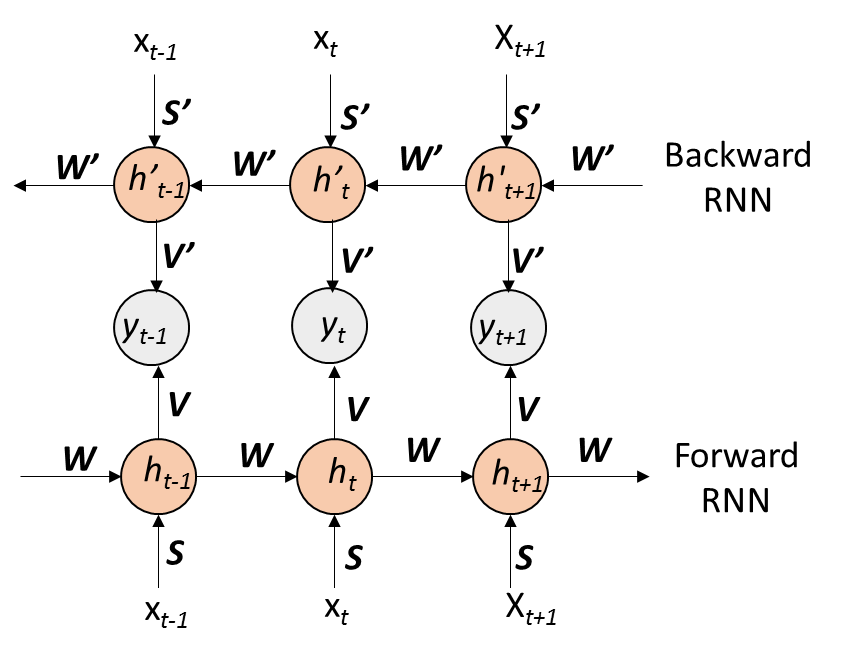
\includegraphics[width=150pt]{figures/bidirectional.png}
		\captionsource{Working of Bi-directional LSTM}{https://subscription.packtpub.com/book/big\_data\_and\_business\_intelligence\\
		/9781787121089/6/ch06lvl1sec69/setting-up-a-bidirectional-rnn-model}
		\label{fig:bidilstm}
	\end{center}
\end{figure}\newline
In the picture, \say{w} is the weights that are updated from taking the sequence in its right order (\say{s}) and \say{w'} are the weights that are updated from the taking the sequence in reverse (\say{s'}). \say{h} and \say{h'} are the hidden nodes for forward and backward sequences respectively and \say{x} and \say{y} are input and output nodes.
From the picture above, the forward RNN is responsible for handling the input data in the usual direction and backward RNN is responsible for the reverse sequence of the input data. Both, the forward and backward LSTM combine to give output for that particular time-step (t-1, t, t+1) or word-step(our case).
\subsection{Lemmatization}
Lemmatization is the process of reducing the words to their root words i.e. \say{asked}, \say{asking} will be reduced to \say{ask}. This mostly helps in reducing the number of unique words but keeping the intent same \cite{Manning:2008:IIR:1394399}. This can be done using the NLTK package which is readily available in python \cite{Loper:2002:NNL:1118108.1118117}.
\subsection{STOP Words}
While working with textual data, there will always be words that occur most frequently but do not contribute significantly to the essence of the text \cite{Manning:2008:IIR:1394399}. Such words are known as STOP words. Removing such words helps in reducing the time spent on indexing the words and helps in concentrating on words that actually contribute to the meaning. This can be done using the NLTK package which is readily available in python. \cite{Loper:2002:NNL:1118108.1118117}
\subsection{Contractions}
 Contractions are shortened words mostly present in spoken vocabulary and ultimately adopted to written. In English, an example of contraction of phrase \say{I have} would be \say{I’ve}. We expand such contractions so that we have some sort of standardization of text \cite{Sarkar:2016:TAP:3086768}. A typical way of dealing with contractions is to make a table of all known contractions and expand all the current contractions we found in the text corpus via the given table. 
 \subsection{Word Embeddings}
 Word embeddings is a natural language modelling technique that turns text into vector representations(made of numbers) of a word. This transformation is necessary because machine learning algorithms require their input to be numbers since the models don't work on strings of plain text. Embeddings map words or phrases from a vocabulary to a corresponding vector of real numbers. Word embeddings are usually used for following properties:
 \begin{itemize}
     \item Dimensionality Reduction: Usually, when dealing with large corpus of textual data, the dimensionality of vectors formed is very large and word embedding aims to create a vector representation of them in a much lower dimensional space \cite{pennington2014glove}. This is achieved effectively by combining PCA based dimensionality reduction with a post-processing algorithm, to construct word embeddings of lower dimensions.\cite{DBLP:journals/corr/abs-1708-03629}
     \item Contextual Similarity: For a language model to be able to predict the meaning of text, it needs to be aware of the contextual similarity of words.\cite{DBLP:journals/corr/MikolovSCCD13}
     A measure of similarity of words can be achieved by taking cosine of the word vectors. The standard comparison metric is cosine similarity, which is equivalent to dot product if the vectors are normalized. Other metrics include Euclidean distance, the less-known Tanimoto similarity, which is similar to cosine similarity but with a different normalization factor.\cite{Thesis}
 \end{itemize}
 \subsection{Class Imbalance}
 Class imbalance refers to the phenomenon where some classes (labels) of a dataset have more samples than others. This is a problem because the machine learning algorithms will tend to focus on the classification of the samples that are over represented while ignoring or misclassifying the underrepresented samples. In our dataset, we have only 80810 samples of insincere questions and 1225312 samples of sincere questions. The classifier will tend to classify insincere questions as sincere ones. There are several methods to overcome this problem:
 \begin{itemize}
     \item Undersampling- Under sampling is a method where we try to extract samples from the main dataset, in a sense to balance the dataset where the no. of target classes have approximately equal no of samples. We remove some of the majority class samples from the dataset in order to balance the majority and minority class samples, so it has less effect on the machine learning algorithm. However, we could risk discarding useful information as some of the majority class instances might be more representative and we run a risk of removing these instances. \cite{Liu:2009:ITC:1453254.1453338}
     \item Oversampling- Instead of removing samples of majority classes, we add more samples of the minority class by replication, so it has more effect on the machine learning algorithm \cite{Liu:2009:ITC:1453254.1453338}. However, just duplicating the minority classes could lead the classifier to overfit a few examples.
     \item SMOTE - An over-sampling approach in which the minority class is over-sampled by creating \say{synthetic} examples rather than by over-sampling with replication \cite{DBLP:journals/corr/abs-1106-1813}. SMOTE iterates over the existing, real minority class instances. At each iteration, it chooses one of the K closest minority class neighbours and synthesizes a new minority instance somewhere between the minority instance and that neighbour. Depending upon the amount of over-sampling required, neighbors from the k nearest neighbors are randomly chosen.
 \end{itemize}
 
 \subsection{Performance Measures}
 Accuracy is not the metric to use when working with an imbalanced dataset. It is very misleading. There are other metrics that give a better story about the performance of the model when working with imbalanced classes such as: Precision, Recall and F1 Score.
 \begin{itemize}
     \item Precision: Precision is the ratio of correctly predicted positive observations to the total predicted positive observations. 
     \item Recall: Recall is the ratio of correctly predicted positive observations to the all observations in sample test data.
     \item F1-Score: F1 Score is the weighted average of Precision and Recall. Therefore, this score takes both false positives and false negatives into account. It is used as a measure between the precision and the recall and gives a sense of how balanced the model is in predicting the right labels in whole of the sample.
 \end{itemize}
 The formula for F1-score is given by $F_{1}=2 \times \frac{\text{precision} \times \text{recall}}{\text{precision} + \text{recall}}$
 \newline
 Intuitively F1 score is not as easy to understand as accuracy, but it is usually more useful than accuracy, especially if you have an uneven class distribution.
\section{Previous Work}
%Whatever is mentioned in the report comments
Many existing models \cite{Kaggle1} on Kaggle were built using Bidirectional Gated Recurrent Unit (GRU) with and without any pre-trained embeddings provided in the dataset. First, the training dataset was split into training and validation samples, with training set holding 90\% of the data and the validation set holding the remaining 10\% data.\\For pre-processing, the model filled up the missing values in the text column with \say{na}. The text column was tokenized and converted into vector sequences. Next, the sequence was padded as needed; if the number of words in the text were greater than the maximum length of the text, then it was truncated to maximum length or if the number of words in the text was less than maximum length, zeros were added for the remaining values.\cite{Kaggle}

\subsection{Model Architecture}
There were two models built and their performances were compared to each other. The models are stated as follows:
\begin{itemize}
		\item Model 1: Without using pre-trained embeddings- The Bidirectional Gated Recurrent Unit (GRU) model was trained using 1 input layer with 128 neurons, embedding of size 300, maximum number of words in a question to be 100 (maximum length), dropout 0.1 and sigmoid as the activation function.
		\item Model 2: Using pre-trained embeddings- The same baseline Bidirectional GRU model (Model 1) was rebuilt using three pre-trained embeddings, namely- Glove, Wiki News FastText and Paragram.
\end{itemize}
Finally the models were compiled using binary cross entropy and \say{adam} optimizer. The models carried out validation set predictions and test set predictions and calculated the F-1 score.

\subsection{Observations}
\begin{itemize}
		\item The pre-trained embeddings model (Model 2) gave better results as compared to non pre-trained embeddings model (Model 1).
		\item The performance of the different pre-trained embeddings used in Model 2 were almost similar to each other.\cite{Kaggle}
\end{itemize}
\section{Proposed Work}
We have tried a bi-directional LSTM with both under sampling and Synthetic Minority Over-sampling (SMOTE) for our experiments. 
\subsection{Pre-Processing}
First, we preprocess the data which involves converting the input to lower case, fixing common contractions, removing punctuation, some common stop words and numbers and then lemmatizing the text. \newline
After preprocessing, we observe that out of 1.3 million sentences, 1.2 million sentences are composed of 10 or less words. Hence, we decided that each input to the model should have 10 words in it. If a sentence has less words, then we pad it with appropriate number of padding text such that the sentence has 10 words otherwise, if a sentence has more than 10 words then we take first 10 words of the sentence under consideration. \newline
Next, we build a dictionary item over this data, which holds all the unique words in our data as the key and a unique integer as its value. Also, we add an extra item to this dictionary as \say{unk} that describes the words that are not present in the training set, but present in the test data.\newline
We split the input dataset into training, validation and test subset to evaluate our model. For this, we first create a test set which contains 10000 samples from the dataset chosen randomly. From the remaining data, we create training and validation set. Our training set holds 80\% of the data and the validation set has the remaining 20\% data.\par
Since, we have a class imbalance problem here, we overcome this by using some sampling. For our experiments, we apply SMOTE and undersampling over the training set and compare the performance of the models trained on the data thus obtained. Our training set initially had 64810 insincere questions and 979762 sincere questions. SMOTE balances the uneven counts and generates dataset with same number of insincere and sincere questions i.e. 979762 samples of each class. SMOTE is proven to be beneficial for synthetic text generation if the input dimensions are not very high. In our case, we have 10-dimensional input data which benefits SMOTE. Similarly, undersampling creates a dataset that comprises of 64810 samples of each class. Using PyTorch Dataloader, we create batches of size 128 for training, test and validation datasets. Now that our data is ready to be fed to the model, we create a basic LSTM model, with two fully connected layer stacked over it. and train it for 20 epochs.\newline
\subsection{Model Architecture}
Our model comprises of 2 Layers of bidirectional LSTMs, each with 512 neurons. We use an embedding layer, which has rows as the number of items in the dictionary created earlier and 300 columns. Further, we use a dropout of 0.5 in the final layer. We average out the forward and backward feed results from the LSTM and then feed it to a fully connected layer which has batch normalization. Batch normalization normalizes the output of a previous activation layer by subtracting the batch mean and dividing by the batch standard deviation. It improves the stability of a neural network. Finally, we apply the sigmoid activation function over the output from previous step which in return gives us the binary text classification for the given input.\newline
\subsection{Finetuning the parameters}
We investigate the following parameters to check the performance of our model:
\begin{itemize}
    \item batch size: 64, 128, 256, 512
    \item optimizers: adam, sgd, adamax, rmsprop, adagrad \cite{DBLP:journals/corr/Ruder16}
    \item learning rate : 0.1, 0.001, 0.0001
    \item activation function : softmax, sigmoid, relu, tanh \cite{eger-etal-2018-time}
    \item dropout : 0.2,0.4,0.5,0.6,0.8 \cite{DBLP:journals/corr/abs-1207-0580}
    \item number of layers for LSTM : 1,2,3,4
\end{itemize}
For this, we train the model using each of these parameters and choose the parameters for which the model performs the best over validation set.
\section{Results and Future Work}
We got the best results with batch size- 128, learning rate- 0.001, dropout- 0.5, num\_layers- 2, activation function- sigmoid, optimizer- adam. The model trained over undersampled data performs poorly over the test data when compared with the model trained over SMOTE sampled data. We were able to achieve 0.95 f1- score performance for majority class and 0.57 f1-score performance for minority class i.e. insincere questions on the test data using these parameters, where the input data fed to the model is sampled used SMOTE.  For the model trained over undersampled data, we get an f1-score of 0.93 for the majority class 0.48 for the minority class.
\begin{figure}[h]
	\begin{center}
		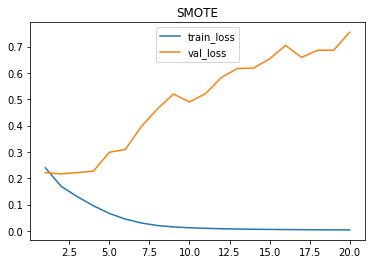
\includegraphics[width=150pt]{figures/smote.png}
		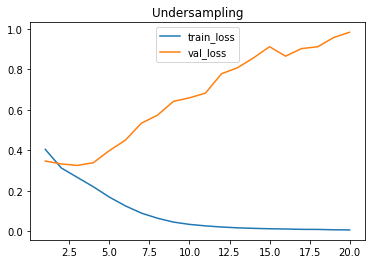
\includegraphics[width=150pt]{figures/undersampling.png}
		\label{fig:Model Performance over SMOTE}
	\end{center}
\end{figure}

Whereas, the existing Model 1 got a F1-score of 0.65 without using any embeddings with activation function- sigmoid, optimizer-adam and metrics- accuracy and the best F1-score of 0.67 using Glove embedding in Model 2. The existing model performed better than our proposed model as it used Gated Recurrent Unit (GRU) which performs better than Long short-term memory (LSTM) used in our model, as GRU is easy to modify and doesn't require memory units, so it trains faster and is much more efficient than LSTMs.

An extension or improvement of our work would be to leverage an attention model to identify which parts of the sequences are holding high information that can help predict the correct class. Also, models using Gated Recurrent Unit (GRU) have shown promising results in identifying the classes with high accuracy and can be used in combination with attention mechanism to achieve better results. 


%for citing any reference add it in the .bib file and cite it using \cite{} command and pass the name which you gave it in .bib file it will be generated in the latex report automatically
\pagebreak
\bibliographystyle{unsrt}
\bibliography{references}
\end{document}
